\documentclass[report]{subfiles}
\begin{document}
\section{On capacitance, MOSFETs, and regions}
%David
We start with nomenclature. There are two basic kinds of MOSFETs\footnote{Metal-Oxide-Semiconductor [what it's made of] Field Effect Transistor [how it works]}: nFETs and pFETs. These are sometimes also called $n$-channel and $p$-channel transistors (respectively), and – in an $n$-well device – native and well transistors (respectively). The nFET has an $n$-type source and drain sitting in a $p$-type substrate, and the pFET is vice-versa.\\ \\
We have devices now – things to plug in. You tie the nFET's drain to a higher voltage than its \textsl{source} (which will \textsl{source} electrons), and the pFET is vice-versa (because it will \textsl{source} holes). ``Source'' and ``drain'' are so named because they respectively \textsl{source} and \textsl{drain} the majority mobile carrier of the given transistor type.\\ \\
You don't want current crossing the $pn$ junctions where the drain and source sit in the substrate, so we reverse bias those junctions\footnote{Put $n$ at a higher voltage than $p$}. That means we stick the nFET bulk to ground (usually hardwired on the chip), and keep $V_s, V_d > 0$. Look at that – we've plugged it in! \\ \\
We know about the sub- and above threshold regions. Moving between these two regions is a function of $V_g$, specifically the voltage between the gate and the source ($V_{gs} = V_g - V_s$). Both the sub- and the above threshold regions are divided into the triode\footnote{Interesting but irrelevant: ``triode'' comes from the original thought behind the transistor as a 3-terminal diode, thus \emph{tri-}ode vs. \emph{di}-ode. The entire transistor history on Wikipedia is a really interesting read.} and saturation regimes. For both sides of the threshold, we move in and out of saturation by changing $V_{ds}$ – the drain-source voltage.\\ \\
\textsl{This is important: changing \emph{gate-source} voltage from low to high moves us from subthreshold to above threshold for \emph{any} $V_{ds} > 0$. Similarly, changing \emph{drain-source} voltage from low to high moves us from ohmic regime to saturation regime for \emph{any} $V_{gs} > 0$.} \\ \\
Surface voltage $\psi_s$ deserves another mention. We've built a transistor, plugged it in, and biased the gate relative to the bulk\footnote{Really, we care about all voltages \emph{relative to the bulk}, but bulk is almost always at ground so it's an implicit relation}. Because of the positive gate voltage, the depletion region does not only surround the drain and source, but also extends between them. Having this channel of depletion region means that there is a built-in voltage across it\footnote{Not across it as in a \emph{drain-source} voltage, but across it as in perpendicular to the plane of the insulating oxide}. So here we have two voltages in series – one across the insulating oxide, one across the depletion region. Current isn't flowing across either of these gradients, so what does that mean? It means static, accumulated charges are hanging out on either side of the gradients. In other words: they are capacitances. The relationship between the capacitances is described by $\kappa$, which we call the \textsl{capacitive coupling ratio} from gate to channel. It describes how effectively a change in gate voltage can change the surface voltage.
%------Transistor cross-section-------
\begin{figure}[hb]
 \centering
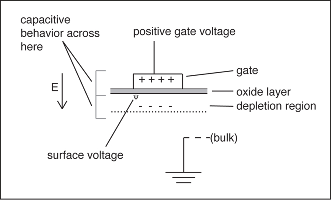
\includegraphics[natwidth=663,natheight=400]{pics/nme_xSection.pdf}
\caption{Cross-section of the transistor gate, oxide layer, and depletion region. When $V_{gate-bulk} > 0$, both the oxide insulator and the depletion region (channel) act as capacitors. See Figure 2.18, p.42 in the textbook for a proper version of this figure.\label{crossSectionCaps}}
\end{figure}
%-----------------------------------------------
%-----------------------------------------------

%Joachim
\subsection{MOSFET Operation Domains}
The operation domain of an nFET is set by the relative values of the four terminals of the transistor.\\
In general, these operation domains (e.g. accumulation) are equivalent to the ones of the MIS structure.\\
We can map the regimes to a MOSFET mode:


\begin{longtable}{ |p{4cm}|p{4cm}|p{4cm}| }
\hline
\textbf{When the MOSFET is in this domain:} & \textbf{We say the MOSFET operates in:} & \textbf{Which can be further divided into (depending on $V_{gs}$:} \\ \hline
\endhead
Accumulation & Cutoff & \\ \hline
Depletion & Cutoff & \\ \hline

Weak Inversion & Subthreshold & Triode Mode \par Saturation Mode\\ \hline
 Strong Inversion & Above Threshold & Triode Mode \par Saturation Mode\\ \hline
\end{longtable}
\end{document}